\chapter{Intrinsic Properties and Scattering Mechanisms}\label{chap:results}
Intro...

\section{Approach to Low-Resistance Contacts}\label{sec:contacts}
Developing low-resistance contacts is important two enable the study of intrinsic transport properties of devices, but also it is vital to applications of \acp{TMD}. Large contact resistance at room temperature is not ideal for applications. At the metal/semiconductor contact interface a barrier develops, the \acs{SB} \cite{Schottky_ZPhys1938}.

In order to address these issues, several approaches to reducing the contact resistance have been probed. 

\subsection{Transmission Line Method: \lightlyfive}\label{subsec:TLM_lightly}
\begin{figure}[ht]
	\centering
	\subfloat[]{
		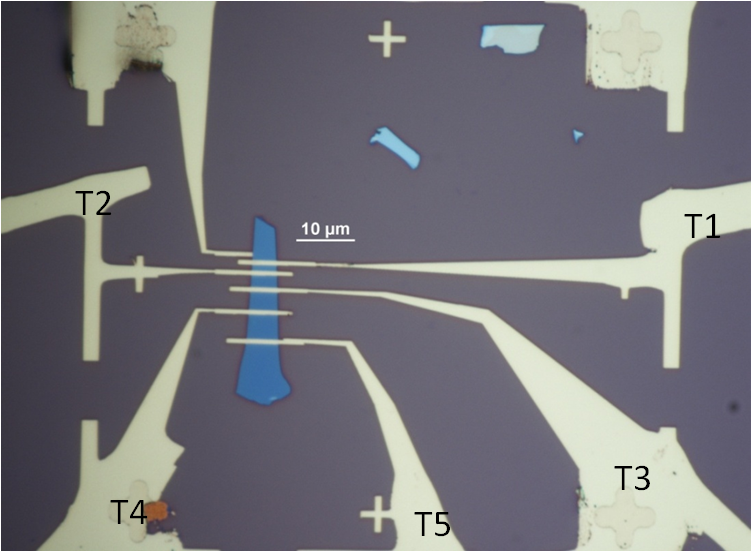
\includegraphics[height=4.25cm,width=5.0cm]{figs/results/transmission_line/transmission_device_pic_5-5_21_10232015_no1}
		\label{fig:transmission_device_10232015_no1}
	}
	\subfloat[]{
		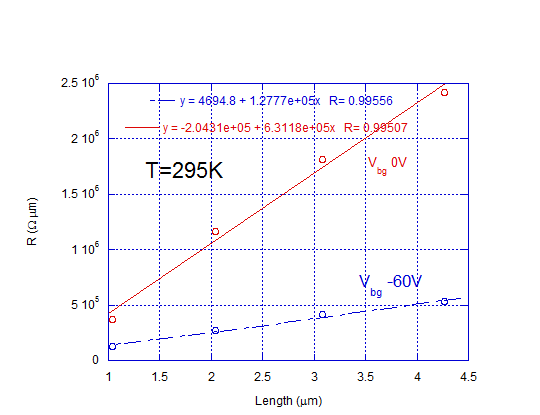
\includegraphics[height=4.25cm,width=5.0cm]{figs/results/transmission_line/transmission_resistance_plot_pic_5-5_21_10232015_no1}
		\label{fig:tlm_resistance1}
	}

	%\qquad
	\subfloat[]{
		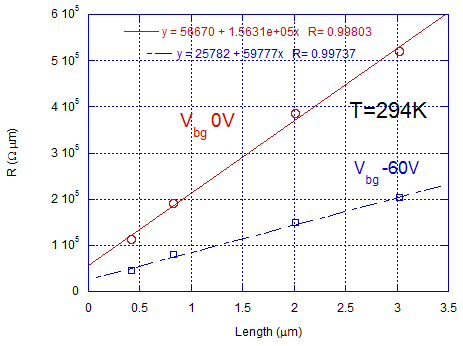
\includegraphics[height=4.25cm,width=5.0cm]{figs/results/transmission_line/transmission_resistance_plot_pic_56_21_10232015_no2}
		\label{fig:tlm_resistance2}
	}
	\subfloat[]{
		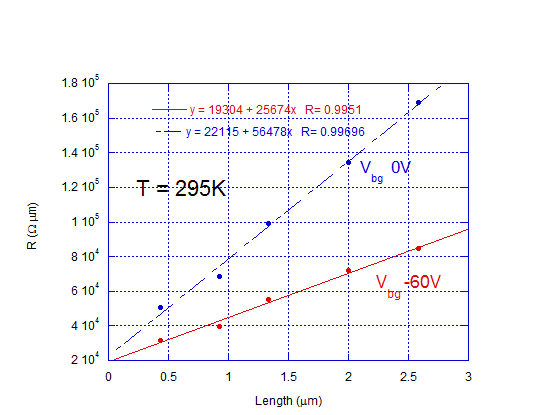
\includegraphics[height=4.25cm,width=5.0cm]{figs/results/transmission_line/transmission_resistance_plot_pic_-66_21_11182015_no2}
		\label{fig:tlm_resistance3}
	}
	\caption[TLM: contact resistances using \lightlyfive]{\protect\subref{fig:transmission_device_10232015_no1} Optical micrograph of a device structure for \acs{TLM} measurement consisting of lightly $p$-doped \ch{WSe2} (\lightlyfive) with \ch{Ti}/\ch{Au} metal contacts. \protect\subref{fig:tlm_resistance1}-\protect\subref{fig:tlm_resistance3} Normalized total resistance as a function of channel length measured at room temperature.}
	\label{fig:tlm_resistance_measurement_lightly}
\end{figure}

\subsection{Transmission Line Method: \degenerate}\label{subsec:TLM_degenerate}
\begin{figure}[ht]
	\centering
	\subfloat[]{
		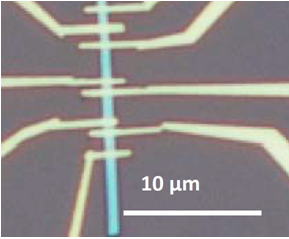
\includegraphics[height=4.25cm,width=5.0cm]{figs/results/transmission_line/ben_tlm_degenerately_doped_device_pic}
		\label{fig:ben_tlm_resistance1}
	}
	%\qquad
	\subfloat[]{
		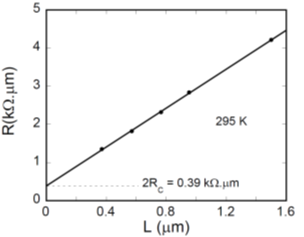
\includegraphics[height=4.25cm,width=5.0cm]{figs/results/transmission_line/ben_tlm_degenerately_doped_resistance_295K}
		\label{fig:ben_tlm_resistance2}
	}
	%\qquad
	\subfloat[]{
		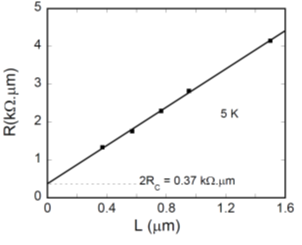
\includegraphics[height=4.25cm,width=5.0cm]{figs/results/transmission_line/ben_tlm_degenerately_doped_resistance_5K}
		\label{fig:ben_tlm_resistance3}
	}
	\caption[TLM: contact resistances using \degenerate]{\protect\subref{fig:ben_tlm_resistance1} Optical micrograph of a device structure for \acs{TLM} measurement consisting of degenerately $p$-doped \ch{WSe2} (\degenerate) with \ch{Ti}/\ch{Au} metal contacts. \protect\subref{fig:ben_tlm_resistance2} Normalized total resistance as a function of channel length measured at room temperature $T=295\unita{K}$ and \protect\subref{fig:ben_tlm_resistance3} low temperature $T=5\unita{K}$. Figures appeared in ref.~\cite{Chuang_2016}.}
	\label{fig:tlm_resistance_measurement_degenerate}
\end{figure}

\begin{table}[ht]
	\centering
	\begin{threeparttable}
		\begin{tabular}{c c c}
			%\hline\hline
			\toprule
			Doping Content & Temperature ($\unita{K}$) & $R_\mathrm{c}(\unita{k\Omega\cdot\mu m})$ \\ [0.5ex]
			%\hline
			\midrule
			$(0.05\%)$ \lightlyfive & 295 & $2.35$\tnote{$\dagger$}\\
			$(0.05\%)$ \lightlyfive & 294 & $12.9$\tnote{$\dagger$}\\
			$(0.05\%)$ \lightlyfive & 295 & $9.65$\tnote{$\dagger$}\\ 
			$(0.5\%)$ \degenerate & 295 & $0.195$\tnote{$\ddagger$}\\ 
			$(0.5\%)$ \degenerate & 5 & $0.185$\tnote{$\ddagger$}\\[1ex]
			%\hline
			\bottomrule
		\end{tabular}
		\begin{tablenotes}
			\item[$\dagger$] Resistance values from figs.~\subref*{fig:tlm_resistance1}, \subref*{fig:tlm_resistance2}, and \subref*{fig:tlm_resistance3}.
			\item[$\ddagger$] Resistance values from figs.~\subref*{fig:ben_tlm_resistance2} and \subref*{fig:ben_tlm_resistance3}.
		\end{tablenotes}
	\caption[Summary of contact resistances lightly $p$-doped and degenerately $p$-doped \ch{WSe2}]{Summary of contact resistances for lightly $p$-doped \ch{WSe2} (\lightlyfive) and degenerately $p$-doped \ch{WSe2} (\degenerate) found using linear fit data from figs.~\subref*{fig:tlm_resistance1}-\subref*{fig:tlm_resistance3}, \subref*{fig:ben_tlm_resistance2}-\subref*{fig:ben_tlm_resistance3}.}
	\label{table:contact_summary}
	\end{threeparttable}
\end{table}

\section{Field-Effect Mobility and Scattering Mechanisms}\label{sec:mufe_scatter}
\begin{figure}[ht]
	\centering
	\subfloat[]{
		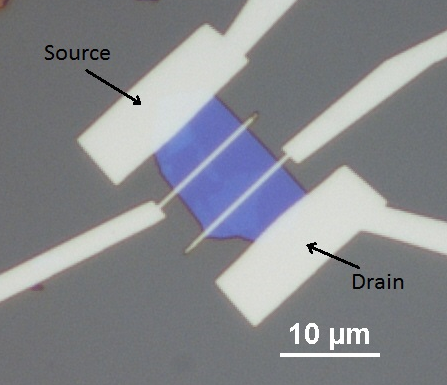
\includegraphics[height=4cm,width=4.75cm]{figs/-44_54_100x_after_liftoff_two_point_probe_measurement}
		\label{fig:two_probe}
	}
	\qquad
	\subfloat[]{
		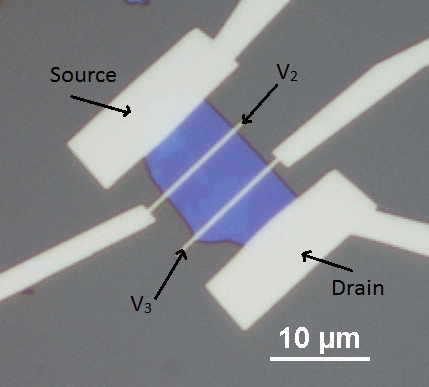
\includegraphics[height=4cm,width=4.75cm]{figs/-44_54_100x_after_liftoff_four_point_measurement}
		\label{fig:four_probe}
	}
	\caption[Field-effect mobility measurement configuration]{Examples of \protect\subref{fig:two_probe} two-point probe measurement configuration for field-effect mobility measurements and \protect\subref{fig:four_probe} four-point probe configuration.}
\end{figure}

\subsection{Applying Low-Resistance Contacts: Doped Channel}\label{subsec:mufe_doped_channel}
\begin{figure}[ht]
	\centering
	\subfloat[]{
		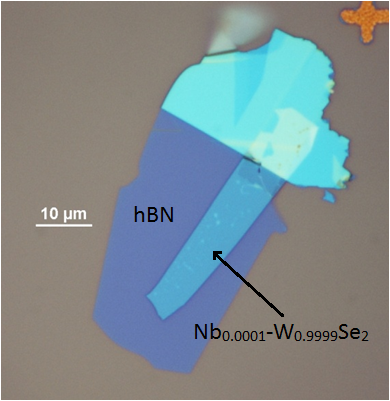
\includegraphics[height=3.75cm,width=3cm]{figs/results/hall_bar_doped_channel_doped_contacts/pWSe2_on_hBN_substrate_5-5_21_no1_annotated}
		\label{fig:pWSe2_doped_contacts_and_channel_step1}
	}
	\qquad
	\subfloat[]{
		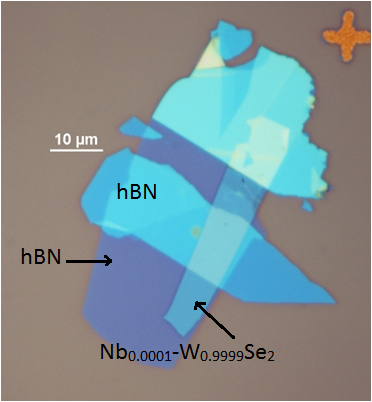
\includegraphics[height=3.75cm,width=3cm]{figs/results/hall_bar_doped_channel_doped_contacts/pWSe2_on_hBN_substrate_with_top_hBN_5-5_21_no1_annotated}
		\label{fig:pWSe2_doped_contacts_and_channel_step2}
	}
	\qquad
	\subfloat[]{
		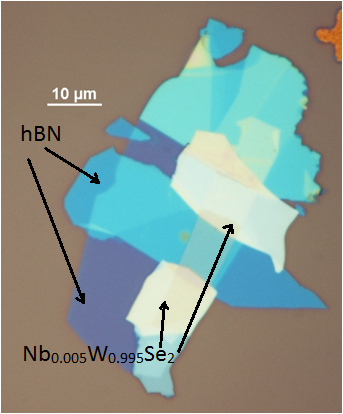
\includegraphics[height=3.75cm,width=3cm]{figs/results/hall_bar_doped_channel_doped_contacts/pWSe2_on_hBN_substrate_with_top_hBN_doped_contact_transfer_5-5_21_no1_annotated}
		\label{fig:pWSe2_doped_contacts_and_channel_step3}
	}
	\qquad
	\subfloat[]{
		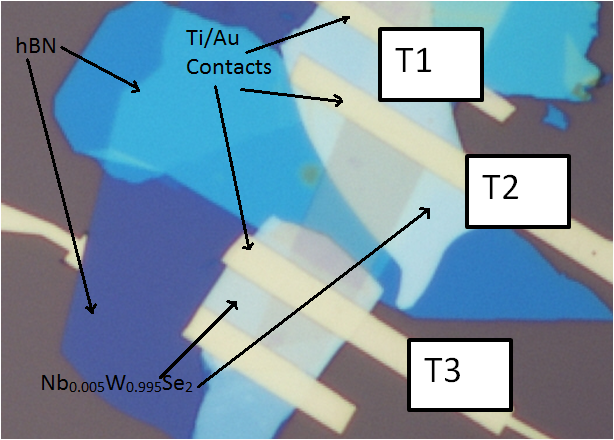
\includegraphics[height=3cm,width=3.75cm]{figs/results/hall_bar_doped_channel_doped_contacts/pWSe2_device_with_electrodes_5-5_21_no1_annotated}
		\label{fig:pWSe2_doped_contacts_and_channel_final_device}
	}
	\caption[Fabrication steps of \lightlyone channel with \degenerate\, contacts]{\protect\subref{fig:pWSe2_doped_contacts_and_channel_step1} \lightlyone transferred to \hbn substate,  \protect\subref{fig:pWSe2_doped_contacts_and_channel_step2} top \hbn transferred onto channel, \protect\subref{fig:pWSe2_doped_contacts_and_channel_step3} degenerately doped (\degenerate) contacts transferred onto device, and \protect\subref{fig:pWSe2_doped_contacts_and_channel_final_device} device after fabrication steps with \ch{Ti}/\ch{Au} metal electrodes consisting of a $5.6\unita{nm}$ thick channel.}
	\label{fig:hBN_field_effect_device_fab}
\end{figure}

\begin{figure}[ht]
	\centering 
	\subfloat[]{
		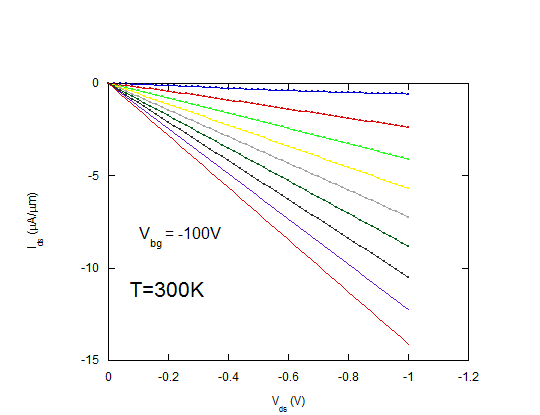
\includegraphics[height=4.55cm,width=5.3cm]{figs/results/hall_bar_doped_channel_doped_contacts/Vds-Id_Vds_1V_-1V-Vbg_-20V_-100V_T2-T3_300K-04_plot_before_anneal_5-5_21_no1}
		\label{fig:5-5_21_no1_pre_anneal_iv_300k}
	}
	\subfloat[]{
		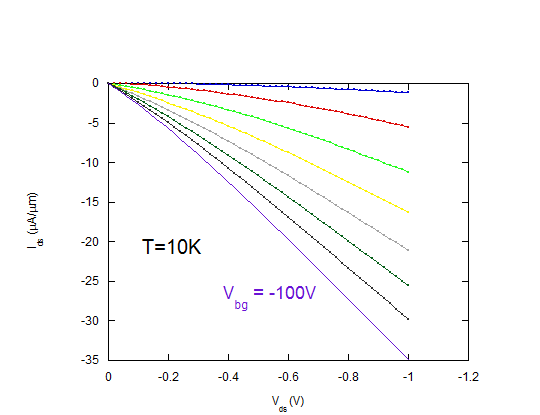
\includegraphics[height=4.55cm,width=5.3cm]{figs/results/hall_bar_doped_channel_doped_contacts/Vds-Id_Vds_1V_-1V-Vbg_-30V_-100V_T2-T3_10K-03_plot_before_anneal_5-5_21_no1}
		\label{fig:5-5_21_no1_pre_anneal_iv_10k}
	}
	\subfloat[]{
		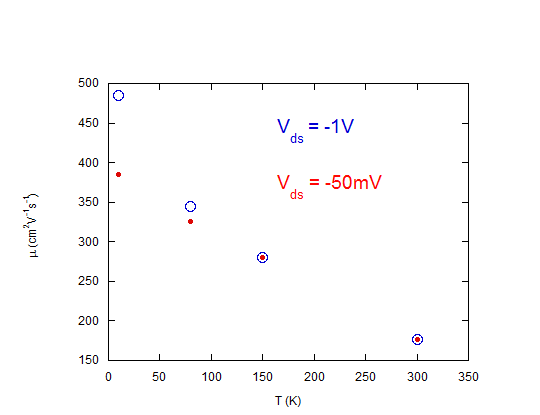
\includegraphics[height=4.55cm,width=5.3cm]{figs/results/hall_bar_doped_channel_doped_contacts/Two_Probe_FE_Mobility_Vs_T_Vds_-1V_-50mV_plot_pre_anneal_5-5_21_no1}
		\label{fig:5-5_21_no1_pre_anneal_mu_fe_vs_temp}
	}
	\caption[Characteristics of \ch{WSe2} \acs{FET} with lightly $p$-doped channel and 2D/2D contacts: I]{\protect\subref{fig:5-5_21_no1_pre_anneal_iv_300k} $IV$ chacteristics of device at $T=300\unita{K}$ and \protect\subref{fig:5-5_21_no1_pre_anneal_iv_10k} at $T=10\unita{K}$. \protect\subref{fig:5-5_21_no1_pre_anneal_mu_fe_vs_temp} Two-terminal field-effect mobility as a function of temperature for $V_{ds}=-50\unita{mV}$ and $-1\unita{V}$. \emph{Note: figures correspond to device shown in fig.~\subref*{fig:pWSe2_doped_contacts_and_channel_final_device}. Measurements shown were made before the device was annealed}.}
	\label{fig:pre_anneal_mu_fe_measurements}
\end{figure}

\begin{figure}[ht]
	\centering
	\subfloat[]{
		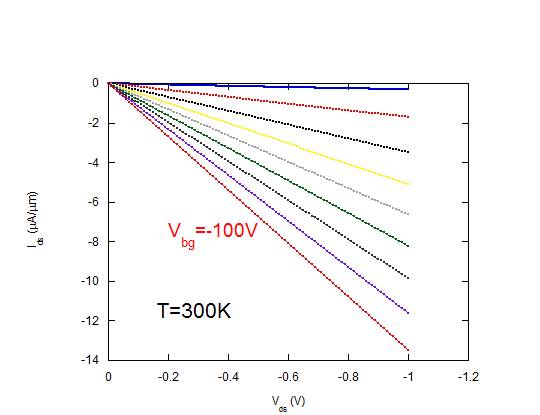
\includegraphics[height=4.55cm,width=5.3cm]{figs/results/hall_bar_doped_channel_doped_contacts/Vds-Id_Vds_1V_-1V-Vbg_-20V_-100V_T2-T3_300K-13_plot_after_anneal_5-5_21_no1}
		\label{fig:5-5_21_no1_post_anneal_iv_300k}
	}
	\subfloat[]{
		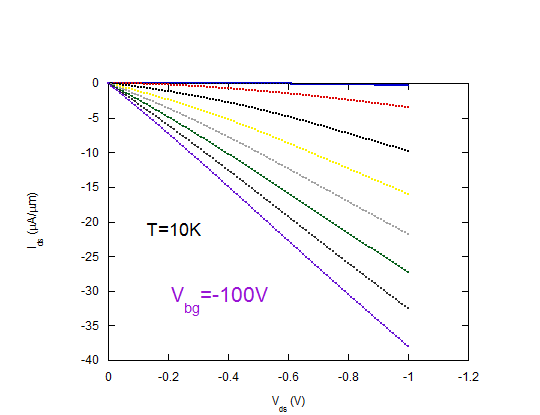
\includegraphics[height=4.55cm,width=5.3cm]{figs/results/hall_bar_doped_channel_doped_contacts/Vds-Id_Vds_1V_-1V-Vbg_-30V_-100V_T2-T3_10K-03_plot_after_anneal_5-5_21_no1}
		\label{fig:5-5_21_no1_post_anneal_iv_10k}
	}
	\subfloat[]{
		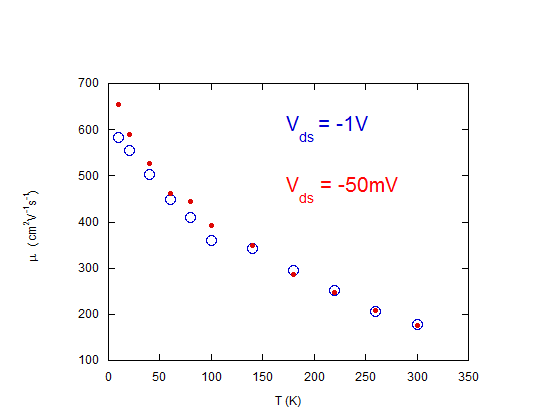
\includegraphics[height=4.55cm,width=5.3cm]{figs/results/hall_bar_doped_channel_doped_contacts/Two_Probe_FE_Mobility_Vs_T_Vds_-1V_-50mV_plot_post_anneal_5-5_21_no1}
		\label{fig:5-5_21_no1_post_anneal_mu_fe_vs_temp}
	}
	\caption[Characteristics of \ch{WSe2} \acs{FET} with lightly $p$-doped channel and 2D/2D contacts: II]{\protect\subref{fig:5-5_21_no1_post_anneal_iv_300k} $IV$ chacteristics of device at $T=300\unita{K}$ and \protect\subref{fig:5-5_21_no1_post_anneal_iv_10k} at $T=10\unita{K}$. \protect\subref{fig:5-5_21_no1_post_anneal_mu_fe_vs_temp} Two-terminal field-effect mobility as a function of temperature for $V_{ds}=-50\unita{mV}$ and $-1\unita{V}$. \emph{Note: figures correspond to device shown in fig.~\subref*{fig:pWSe2_doped_contacts_and_channel_final_device}. Measurements shown weree made after the device was annealed for 30 minutes at $250^\degree\unita{C}$}.}
	\label{fig:post_anneal_mu_fe_measurements}
\end{figure}

\subsection{Applying Low-Resistance Contacts: Undoped Channel}\label{subsec:mufe_undoped_channel}
\begin{figure}[ht]
	\centering
	\subfloat[]{
		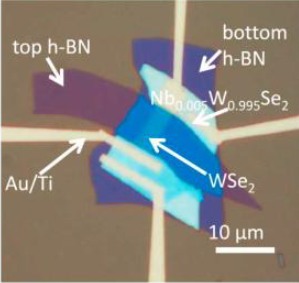
\includegraphics[height=4.5cm,width=5cm]{figs/results/ben/undoped_wse2_degen_doped_contacts}
		\label{fig:undoped_wse2_pic}
	}
	\subfloat[]{
		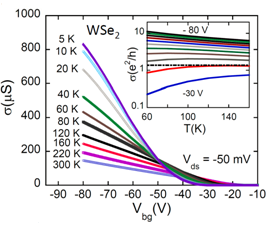
\includegraphics[height=4.5cm,width=5cm]{figs/results/ben/conductivity_2d2d_contacts_vs_Vbg_wse2}
		\label{fig:undoped_wse2_conduct}
	}
	\subfloat[]{
		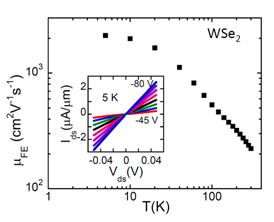
\includegraphics[height=4.5cm,width=5cm]{figs/results/ben/mu_fe_2d2d_contacts_vs_T_wse2}
		\label{fig:undoped_wse2_mu_fe}
	}
	\caption[Characteristics and channel properties of \ch{WSe2} \acs{FET} with 2D/2D contacts]{\protect\subref{fig:undoped_wse2_pic} Optical micrograph of \ch{WSe2} \acs{FET} with degenerately $p$-doped \ch{WSe2} (\degenerate) contacts with channel region on \hbn substrate and covered with a top \hbn piece. \protect\subref{fig:undoped_wse2_conduct} Temperature dependent two-terminal conductivity as a function of $V_{bg}$ at $V_{ds}=-50\unita{mV}$ for device shown in \protect\subref{fig:undoped_wse2_pic}. \protect\subref{fig:undoped_wse2_mu_fe} Two-terminal field-effect mobility. Figures appeared in ref.~\cite{Chuang_2016}.}
	\label{fig:mu_fe_data_degenerate}
\end{figure}

\section{Hall Effect and Applying Low-Resistance Contacts}\label{sec:hall_effect_intro}
\begin{figure}[ht]
	\centering
	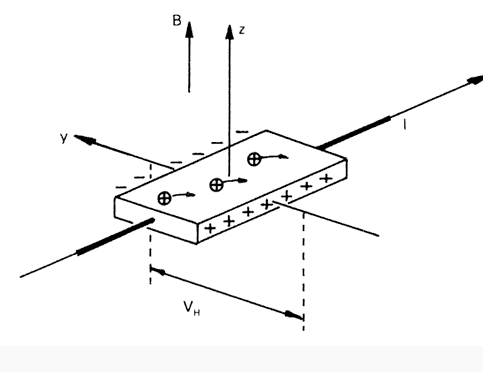
\includegraphics[height=6cm,width=8cm]{figs/results/hall_diagram}
	\caption[Hall effect measurement diagram]{Geometry of Hall effect measurement. Current flows in the positive $x$-direction and magnetic field is applied in the positive $z$ direction generating a Hall voltage \cite{HallEffectNIST}. Diagram originally appeared in ref.~\cite{HallDiagram}.}
	\label{fig:hall_diagram}
\end{figure}

\subsection{Hall Effect: \lightlyfive}\label{subsec:hall_lightly}
\begin{figure}[ht]
	\centering
	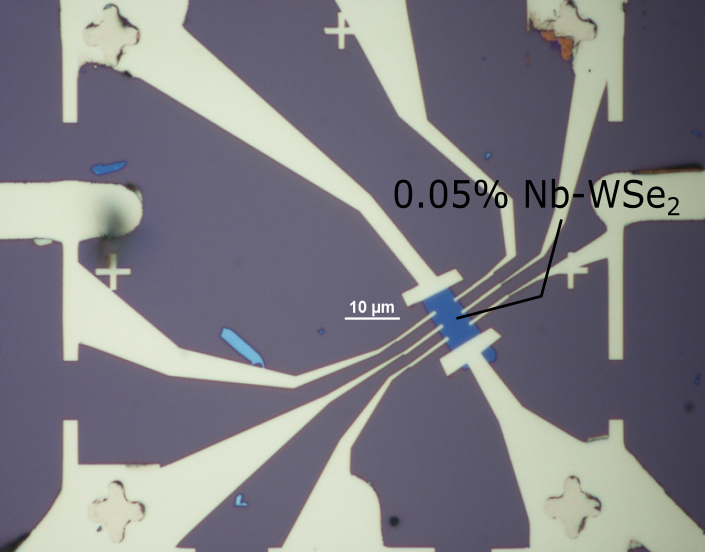
\includegraphics[height=4.5cm,width=6.0cm]{figs/results/hall_bar_doped_channel/hall_bar_device_pic_11192015_no2_doping_scheme}
	\caption[Hall bar device optical micrograph using \lightlyfive]{Optical micrograph of device structure consisting of lightly $p$-doped \ch{WSe2} (\lightlyfive) with device thickness $7.7\unita{nm}$ and \ch{Ti}/\ch{Au} metal contacts.}
	\label{fig:hall_bar_device1}
\end{figure}

\begin{figure}[ht]
	\centering
	\subfloat[]{
		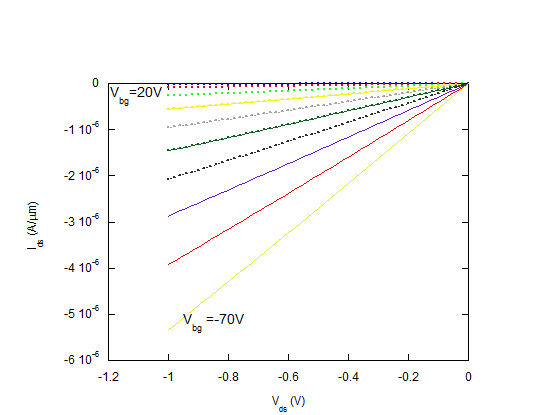
\includegraphics[height=4.25cm,width=5.0cm]{figs/results/hall_bar_doped_channel/Vds-Id_1V_-1V-Vbg_20V_-70V_T1-D_T5_S_300K_plot_modified_11192015_no2}
		\label{fig:11192015_ohmic_contacts}
	}
	%\qquad
	\subfloat[]{
		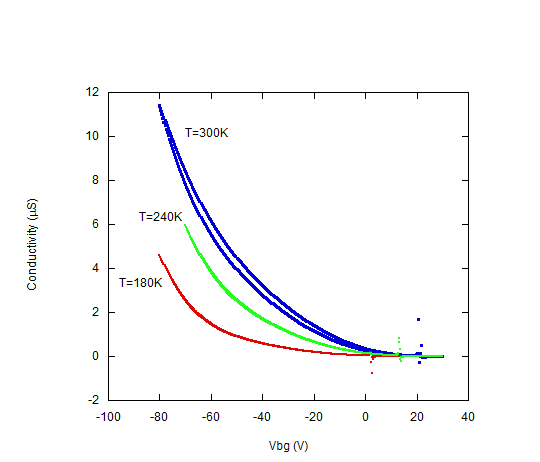
\includegraphics[height=4.25cm,width=5.0cm]{figs/results/hall_bar_doped_channel/hall_bar_device_pic_11192015_no1_conduct_vs_Vbg_all_temps}
		\label{fig:11192015_conduct_vs_temp}
	}
	\subfloat[]{
		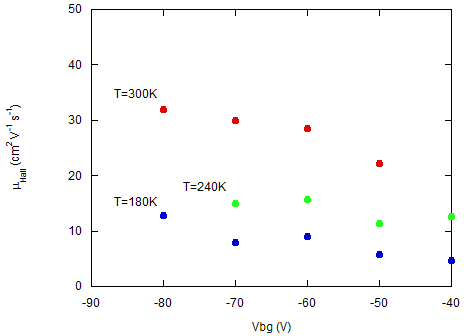
\includegraphics[height=4.25cm,width=5.0cm]{figs/results/hall_bar_doped_channel/hall_bar_device_pic_11192015_no1_mu_hall_vs_Vbg_all_temps}
		\label{fig:11192015_mu_hall_vs_temp}
	}

	%\qquad
	\subfloat[]{
		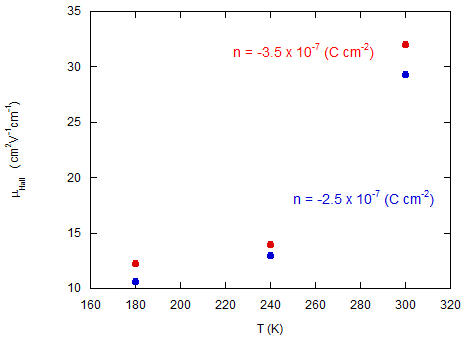
\includegraphics[height=4.25cm,width=5.0cm]{figs/results/hall_bar_doped_channel/HallMobility_Vs_T_for_fixed_carrier_consentrations_plot_modified_11192015_no2}
		\label{fig:11192015_mu_hall_vs_temp_various_n}
	}
	\qquad
	\subfloat[]{
		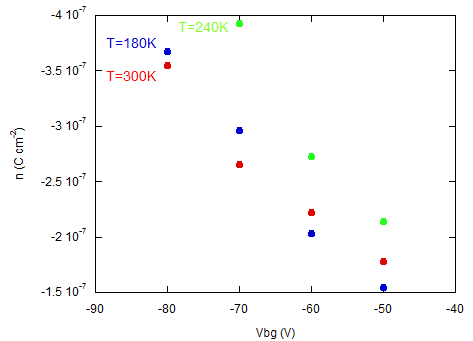
\includegraphics[height=4.25cm,width=5.0cm]{figs/results/hall_bar_doped_channel/Charge_density_Vs_Vbg_different_Temp_plot_modified_11192015_no1}
		\label{fig:11192015_n_vs_Vbg}
	}
	\caption[Output characteristics and channel properties of lightly $p$-doped \ch{WSe2} with 2D/2D contacts]{\protect\subref{fig:11192015_ohmic_contacts} $IV$ characteristic curve at $T=300\unita{K}$ as a function of $V_{ds}$ for $V_{bg}$ ranging from $-70\unita{V}$ to $20\unita{V}$. \protect\subref{fig:11192015_conduct_vs_temp} Temperature-dependence of conductivity and \protect\subref{fig:11192015_mu_hall_vs_temp} Hall mobility as a function of $V_{bg}$. \protect\subref{fig:11192015_mu_hall_vs_temp_various_n} Charge carrier denisty dependence of Hall mobility as a function of temperature and \protect\subref{fig:11192015_n_vs_Vbg} temperature dependence of charge carrier density as a function of $V_{bg}$. \emph{Note: the data here corresponds to device shown in fig.~\ref{fig:hall_bar_device1}}.}
	\label{fig:hall_measurement_data_lightly}
\end{figure}

\subsection{Hall Effect: Extended to Contact Method}\label{subsec:hall_degenerate}

\begin{figure}[ht]
	\centering
	\subfloat[]{
		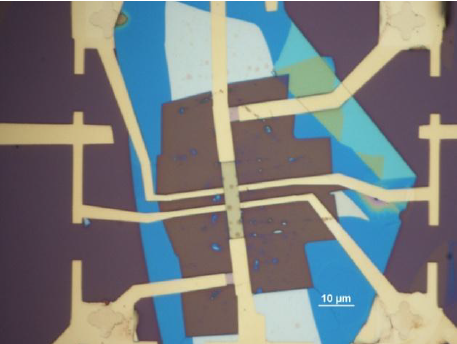
\includegraphics[height=4.75cm,width=5.5cm]{figs/results/ben/pWSe2_hall}
		\label{fig:pWSe2_hall}
	}
	\qquad
	\subfloat[]{
		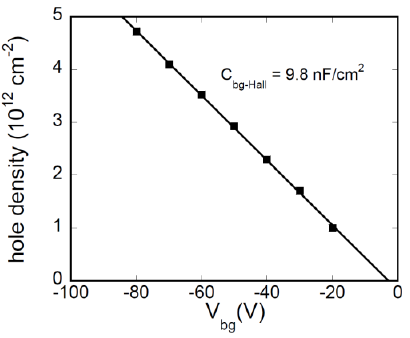
\includegraphics[height=4.75cm,width=5.5cm]{figs/results/ben/pWSe2_cap}
		\label{fig:pWSe2_cap}
	}
	\caption[Hall effect measurement with 2D/2D contacts to determine capacitance]{\protect\subref{fig:pWSe2_hall} Optical microgrpah of \ch{WSe2} Hall bar device encapsulated in \hbn with degenerate 2D/2D contacts. \protect\subref{fig:pWSe2_cap} Hole density as a function of $V_{bg}$ at $T=300\unita{K}$ extracted from Hall effect measurement. Figures appeared in ref.~\cite{Chuang_2016}.}
	\label{fig:pWSe2_hall_ben}
\end{figure}